\documentclass[12pt]{article}

% Layout.
\usepackage[top=1in, bottom=0.75in, left=1in, right=1in, headheight=1in, headsep=6pt]{geometry}

% Fonts.
\usepackage{mathptmx}
\usepackage[scaled=0.86]{helvet}
\renewcommand{\emph}[1]{\textsf{\textbf{#1}}}

% TiKZ.
\usepackage{tikz, pgfplots}
\usetikzlibrary{calc}
\pgfplotsset{compat = newest}
\pgfplotsset{my style/.append style={axis x line=middle, axis y line=
middle, xlabel={$x$}, ylabel={$y$}, axis equal }}

% Misc packages.
\usepackage{amsmath,amssymb,latexsym}
\usepackage{graphicx}
\usepackage{array}
\usepackage{xcolor}
\usepackage{multicol}
\usepackage{enumerate}

% Commands to set various header/footer components.
\makeatletter
\def\doctitle#1{\gdef\@doctitle{#1}}
\doctitle{Use {\tt\textbackslash doctitle\{MY LABEL\}}.}
\def\docdate#1{\gdef\@docdate{#1}}
\docdate{Use {\tt\textbackslash docdate\{MY DATE\}}.}
\def\doccourse#1{\gdef\@doccourse{#1}}
\let\@doccourse\@empty
\def\docscoring#1{\gdef\@docscoring{#1}}
\let\@docscoring\@empty
\def\docversion#1{\gdef\@docversion{#1}}
\let\@docversion\@empty
\makeatother

% Headers and footers layout.
\makeatletter
\usepackage{fancyhdr}
\pagestyle{fancy}
\fancyhf{}
\lhead{\baselineskip 30pt
\emph{\@docdate\hfill\@doctitle}
\ifnum \value{page} > 1\relax\else\\
\emph{Name: \rule{3.5in}{1pt}\hfill \@docscoring}\fi}
\rfoot{\emph{\@docversion}}
\lfoot{\emph{\@doccourse}}
\cfoot{\emph{\thepage}}
\renewcommand{\headrulewidth}{0pt}
\makeatother

% Paragraph spacing
\parindent 0pt
\parskip 6pt plus 1pt

% Problem counters
\newcounter{probcount}
\newcounter{subprobcount}
\setcounter{probcount}{0}

\newcommand{\problem}[1]{%
\par\addvspace{4pt}%
\setcounter{subprobcount}{0}%
\stepcounter{probcount}%
\makebox[0pt][r]{\emph{\arabic{probcount}.}\hskip1ex}\emph{[#1 points]}\hskip1ex}

\newenvironment{subproblems}{%
\begin{enumerate}%
\setcounter{enumi}{\value{subprobcount}}%
\renewcommand{\theenumi}{\emph{\alph{enumi}}}}%
{\setcounter{subprobcount}{\value{enumi}}\end{enumerate}}

% Blanks
\newcommand{\blank}[1]{\rule{#1}{0.5pt}}
\newcommand{\mblank}[1]{\underline{\hspace{#1}}}

% Display helpers
\renewcommand{\d}{\displaystyle}
\newcommand{\ds}{\displaystyle}

% Document info
\doctitle{Math F251X: Quiz 4}
\docdate{February 5, 2026}
\doccourse{UAF Calculus I}
\docversion{Spring 2026}
\docscoring{\blank{0.8in} / 25}

\begin{document}

\emph{Please circle your instructor's name:}
\hfill James Gossell \hfill Gordon Williams \\

There are 25 points possible on this quiz.
Any outside materials are not allowed.
\emph{For full credit, show all work clearly.}

%------------------------------------------------
\problem{10}
The {\bf derivative} of $f(x)$ is defined as follows:
$$f'(x)=\lim_{h\to 0}\frac{f(x+h)-f(x)}{h}.$$
\begin{subproblems}
\item Use the definition of the derivative (above) to find the derivative of the function $\displaystyle f(x)=\frac{2}{\sqrt{x}}$. Use proper limit notation. \emph{No credit will be awarded for finding the derivative via other methods.}
\vfill
\item Use your answer in part (a) to find the equation of the tangent line to $\displaystyle f(x)=\frac{2}{\sqrt{x}}$ at the point $(4,1)$. \emph{Simplify your answer.}
\end{subproblems}
\vspace{2in}
\newpage
\problem{6} The graph of $f(x)$ is shown below. On the \emph{other set of axes}, sketch the graph of $f'(x)$. If there are any asymptotes, draw them with dashed lines. Use open circles to show points where the derivative is not defined, if any. (You are not given values on the $y$-axis; I am interested in the correct shape/holes/asymptotes of the derivative, not the specific values.)
\begin{center}
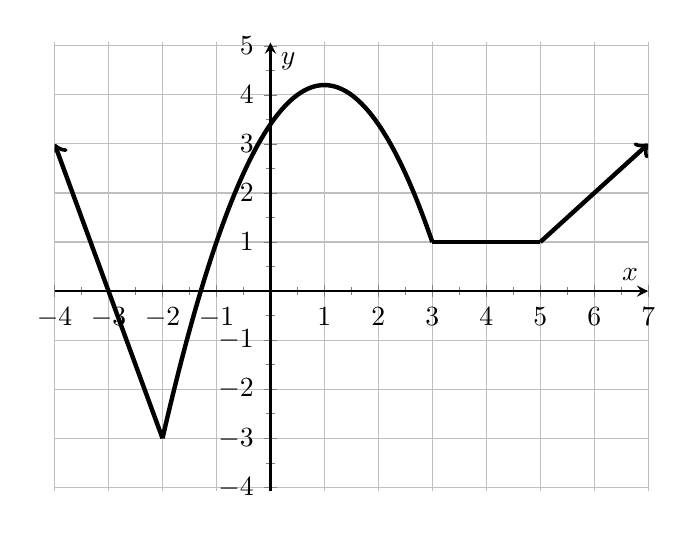
\begin{tikzpicture}
%cubic
\begin{axis}[xscale=1.1, thick, my style, xtick={-4,-3,-2,...,3,4,5, 6, 7}, ytick={-4,-3,...,5},xmin=-4, xmax=7, ymin=-4, ymax=5, minor y tick num=1, minor x tick num=1, 
mark size=3.0pt, grid = major]
\addplot[ultra thick, ->,domain=-4:-1, samples=100]coordinates{(-2,-3)(-4,3)};
\addplot[ultra thick,domain=-2:3, samples=100,-]{(-4*x^2+8*x+17)/5};
%\addplot[ultra thick,domain=-1:2, samples=100, -]{4};
%\addplot[ultra thick, ->,domain=2:7, samples=100]{-(2.6*(x-2)^(1/2))+4}
\addplot[ultra thick, domain=3:5, samples=100]{1};
\addplot[ultra thick, ->,domain=-4:-1, samples=100]coordinates{(5,1)(7,3)};
\end{axis}
\end{tikzpicture}%
\hfill
\begin{tikzpicture}
\begin{axis}[xscale=1.1, thick, my style, xtick={-4,-3,-2,...,3,4,5, 6, 7}, ytick={0},
xmin=-4, xmax=7, ymin=-4, ymax=5, minor y tick num=0, minor x tick num=1, 
mark size=3.0pt, grid = none]
\end{axis}
\end{tikzpicture}
\end{center}
\problem{9} Find $f'(x)$ for each function below. You may use any method you like, and you do not need to simplify your answer.
\begin{subproblems}
\item $f(x)=\displaystyle\frac{8x^{3}-2\sqrt{x}}{x}-\frac{1}{\pi x}$ \hfill({\it Hint: Make it easier, first.})
\vfill
\item $f(x)=(3x^{2}+x)\sin(x)$
\vfill
\item $f(x)=\displaystyle\frac{3\cos(x)}{2^{5}+7x}$
\vfill
\end{subproblems}


%
%\begin{subproblems}
%\begin{multicols}{3}
%\item $\d \lim_{x \to -4^-} f(x) = \mblank{.5in}$
%\item $\d \lim_{x \to -4^+} f(x) = \mblank{.5in}$
%\item $\d \lim_{x \to -4} f(x) = \mblank{.5in}$
%\end{multicols}
%
%\begin{multicols}{3}
%\item $\d \lim_{x \to 2^+} f(x) = \mblank{.5in}$
%\item $\d f(4) = \mblank{.5in}$
%\item $\d \lim_{x \to 4} f(x) = \mblank{.5in}$
%\end{multicols}



\end{document}